\let\negmedspace\undefined
\let\negthickspace\undefined
\documentclass[journal,12pt,twocolumn]{IEEEtran}
\usepackage{cite}
\usepackage{amsmath,amssymb,amsfonts,amsthm}
\usepackage{algorithmic}
\usepackage{graphicx}
\usepackage{textcomp}
\usepackage{xcolor}
\usepackage{txfonts}
\usepackage{listings}
\usepackage{enumitem}
\usepackage{mathtools}
\usepackage{gensymb}
\usepackage{comment}
\usepackage[breaklinks=true]{hyperref}
\usepackage{tkz-euclide} 
\usepackage{listings}
\usepackage{gvv}                                        
\def\inputGnumericTable{}                                 
\usepackage[latin1]{inputenc}                                
\usepackage{color}                                            
\usepackage{array}                                            
\usepackage{longtable}                                       
\usepackage{calc}                                             
\usepackage{multirow}                                         
\usepackage{hhline}                                           
\usepackage{ifthen}                                           
\usepackage{lscape}
\newtheorem{theorem}{Theorem}[section]
\newtheorem{problem}{Problem}
\newtheorem{proposition}{Proposition}[section]
\newtheorem{lemma}{Lemma}[section]
\newtheorem{corollary}[theorem]{Corollary}
\newtheorem{example}{Example}[section]
\newtheorem{definition}[problem]{Definition}
\newcommand{\BEQA}{\begin{eqnarray}}
\newcommand{\EEQA}{\end{eqnarray}}
\newcommand{\define}{\stackrel{\triangle}{=}}
\theoremstyle{remark}
\newtheorem{rem}{Remark}
\begin{document}
\bibliographystyle{IEEEtran}
\vspace{3cm}
\title{\textbf{12.10.6}}
\author{EE23BTECH11040-MANOJ KUMAR AMBATIPUDI$^{*}$% <-this % stops a space
}
\maketitle
\newpage
\bigskip
\renewcommand{\thefigure}{\theenumi}
\renewcommand{\thetable}{\theenumi}
\textbf{Question:}
\\
A beam of light consisting of two wavelengths, 650 nm and 520 nm, is used to
obtain interference fringes in a Young\text{'}s double-slit experiment.\\
(a) Find the distance of the third bright fringe on the screen from
the central maximum for wavelength 650 nm.\\
(b) What is the least distance from the central maximum where the
bright fringes due to both the wavelengths coincide?
\\
\textbf{Solution:}
\\
Let the wave equations of the 2 waves coming from $\lambda_1$ source be $y_1$,$y_2$. Let the wave equations of the 2 waves coming from $\lambda_2$ source be $y_3$,$y_4$, 
\begin{align}
    y_1 &= A_1\sin(2\pi f_1t) \\
    y_2 &= A_1\sin(2\pi f_1t+\phi_1+\phi_2)\\
    y_1 &= A_2\sin(2\pi f_2t) \\
    y_2 &= A_2\sin(2\pi f_2t+\phi_3+\phi_4)
\end{align}
Where $\phi_1,\phi_2,\phi_3,\phi_4$ are phase differences arisen because of position of source.\\
\begin{figure}[h!]
\renewcommand\thefigure{1}
\centering
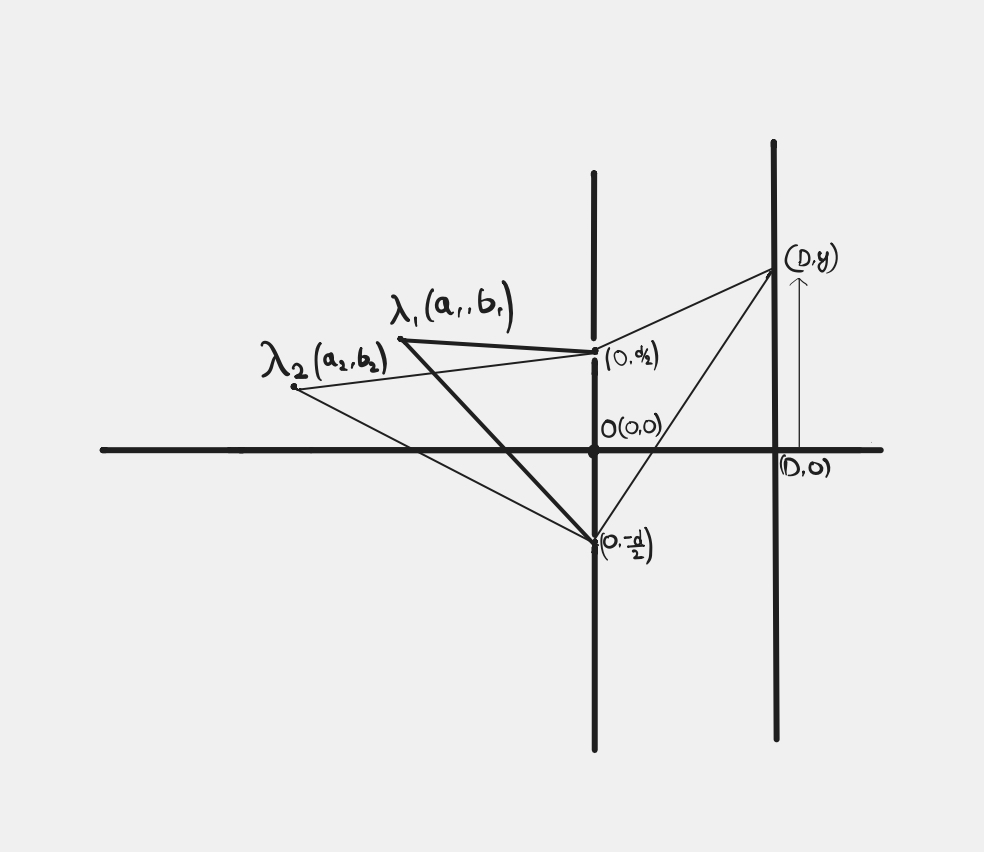
\includegraphics[width=1.0\linewidth]{Fig_5.jpg}
\caption{YDSE SETUP}
\label{fig:enter-label}
\end{figure}
\\
Using principle of superposition, we get 
\begin{align}
    y &= y_1+y_2\\ 
    Y &= y_3+y_4\\
\implies y=&A_1(\sin(2\pi f_1t)+\sin(2\pi f_1t+\phi_1+\phi_2))\\
\implies Y=&A_2(\sin(2\pi f_2t)+\sin(2\pi f_2t+\phi_3+\phi_4))
\end{align}
using
\begin{align}
    \sin(c)+\sin(d)=2\sin(\dfrac{c+d}{2})cos(\dfrac{c-d}{2})
\end{align}
we get
\begin{align}
    y&=2A_1\sin(2\pi f_1t + \dfrac{\phi_1+\phi_2}{2})cos(\dfrac{\phi_1+\phi_2}{2})\\
    Y&=2A_2\sin(2\pi f_2t + \dfrac{\phi_3+\phi_4}{2})cos(\dfrac{\phi_3+\phi_4}{2})
\end{align}
Now for constructive interference to happen,
\begin{align*}
    \\cos(\dfrac{\phi_1+\phi_2}{2})=\pm1 \text{ and } \\cos(\dfrac{\phi_3+\phi_4}{2})=\pm1 
\end{align*}
\begin{align}
\implies \phi_1+\phi_2=2n_1\pi \text{ and } \phi_3+\phi_4=2n_2\pi \label{12.10.6.1}
\end{align}
path difference in terms of phase difference is
\begin{align}
    \Delta x=\Delta\phi\dfrac{\lambda}{2\pi}
\end{align}
Consider wave from $\lambda_1$ source. The phase difference $\phi_1,\phi_2$ corresponding path differences are calculated as  
\begin{align}
    \Delta x_1 &=\sqrt{\brak{\dfrac{d}{2}+b_1}^{2}+(a_1)^{2}} - \sqrt{\brak{\dfrac{d}{2}-b_1}^{2}+(a_1)^{2}}\\
    \Delta x_2 &=\sqrt{\brak{\dfrac{d}{2}+y}^{2}+(D)^{2}} - \sqrt{\brak{\dfrac{d}{2}-y}^{2}+(D)^{2}}
\end{align}
Assuming the approximations 
\begin{align}
    b_1&<<a_1\\
    b_1&\sim d\\
    d&<<D\\
    \brak{1+x}^{n}&\simeq1+nx
\end{align}
We get
\begin{align}
    \Delta x_1 &= \dfrac{db_1}{a_1}\\
    \Delta x_2 &= \dfrac{dy}{D}\\
\end{align}
similarly, path difference of $\lambda_2$ source is
\begin{align}
    \Delta x_3 &= \dfrac{db_2}{a_2}
\end{align}
The sign of path difference is based on the positioning of sources.\brak{\tabref{12.10.6.2}}\\
Depending on the condition, we use appropriate sign convention and calculate path difference as
\begin{align}
    \Delta x = \Delta x_1 + \Delta x_2
\end{align}
for $\lambda_1$ source and
\begin{align}
    \Delta x = \Delta x_3 + \Delta x_2
\end{align}
for $\lambda_2$ source. \\

(a) Finding the distance of the third bright fringe on the screen from the central maximum for wavelength
\begin{align}
\lambda_1 = 650 \, \text{nm}
\end{align}
The path difference for constructive interference is given by:
\begin{align}
\Delta x_1 = n_1\lambda_1     
\end{align}
where  $n_1$ = 3  for the third bright fringe.

Substitute the values:
\begin{align}
\Delta x_1 &= 3\times650 = 1950 \, \text{nm} \\
y_1 &= \Delta x_1\cdot\dfrac{D}{d} = 1950\times\dfrac{D}{d}
\end{align}

(b) The least distance from the central maximum where the bright fringes due to both wavelengths coincide:
Given \[\lambda_1 = 650 \text{nm} ,\lambda_1 = 520 \text{nm}\]
\begin{align}
  n_1 \lambda_1 &= n_2\lambda_2 \\
\frac{n_2}{n_1} &= \frac{\lambda_1}{\lambda_2} = \frac{650}{520}\\
\frac{n_2}{n_1} &= \frac{5}{4}
\end{align}
Now we can assume $n_2$ = 5k and $n_1$ = 4k where k is some positive integer.\\
For smallest value of $y_1$ we shall take k=1.\\
Path difference $\Delta x_1 = 4\times650 = 2600 \text{nm}$\\\\
Now $y_1 =\Delta x_1 \dfrac{D}{d} = 2600\dfrac{D}{d}nm $\\
\textbf{Answer for (b):}
\\
\begin{table}[h!]
\renewcommand\thetable{1}
    \centering
    \begin{tabular}{|c|c|c|}
    \hline
       \textbf{Variable}& \textbf{Description}& \textbf{Value}\\\hline
         $y_1$& Wave Equation of First Wave&none\\\hline
          $y_2$&Wave Equation of Second Wave &none\\\hline
         $y$&   Resultant Wave&none\\\hline
          $f_c$& Frequency of waves&none\\\hline
         $A_1$& Amplitude of First Wave&none\\\hline
         $A_2$& Amplitude of Second Wave&none\\\hline
         $\phi_1$,$\phi_2$& Phase Difference(before Interference)&none\\\hline
         $I_{net}$& Intensity after interference&none\\\hline
         $n_1,n_2$& Non Negative Integer Values&0,1,2....\\\hline
         $\Delta x_1$,$\Delta x_2$& Path Differences&In soln.\\\hline
         $\lambda_{1}$,$\lambda_2$& Wavelengths&650,520\\\hline
         $y_1,y_2$& Distance between central maxima and point&In soln.\\\hline
         $d$& distance between the slits&None\\\hline
         $D$& Distance between Slits and Screen&None\\\hline
         $\theta_1,\theta_2$& Angular Distance From Central Maxima&None\\\hline
    \end{tabular}
    \vspace{0.3cm}
    \caption{\textbf{VARIABLES AND THEIR VALUES}}
    \label{tab:my_label}
\end{table}
\begin{table}[h!]
\renewcommand\thetable{2}
    \centering
    \begin{tabular}{|c|c|c|}
    \hline
         $\Delta x$ measured on $x<0,y<0$&$ -ve $\\\hline
         $\Delta x$ measured on $x<0,y>0$&$ +ve $\\\hline 
    \end{tabular}
    \vspace{0.2cm}
    \caption{\textbf{SIGN CONVENTION FOR PATH DIFFERENCE}}
    \label{12.10.6.2}
\end{table}
\end{document}
